\documentclass{VUMIFPSkursinis}
\usepackage{algorithmicx}
\usepackage{algorithm}
\usepackage{algpseudocode}
\usepackage{amsfonts}
\usepackage{amsmath}
\usepackage{bm}
\usepackage{caption}
\usepackage{color}
\usepackage{float}
\usepackage{graphicx}
\usepackage{listings}
\usepackage{subfig}
\usepackage{wrapfig}
\usepackage{enumitem}

% Titulinio aprašas
\university{Vilniaus universitetas}
\faculty{Matematikos ir informatikos fakultetas}
\department{Programų sistemų katedra}
\papertype{Naudotojų poreikių ir užduočių analizė}
\title{ParQR - Parkavimo mobilioji programėlė}
\titleineng{ParQR - Parking phone app}
\status{3 kurso 5 grupės studentai}
\author{Miglė Vaitulevičiūtė}
\secondauthor{Emilis Ruzveltas}   % Pridėti antrą autorių
\thirdauthor{Justas Žilinskas}   % Pridėti trečią autorių
\fourthauthor{Vytautas Žilinas}   % Pridėti ketvirtą autorių
\supervisor{dr. Kristina Lapin}
\date{Vilnius – \the\year\\Versija 1.0}

% Nustatymai
% \setmainfont{Palemonas}   % Pakeisti teksto šriftą į Palemonas (turi būti įdiegtas sistemoje)
\bibliography{bibliografija}

\begin{document}
\pagenumbering{gobble}
\maketitle

\tableofcontents
\pagenumbering{arabic}
\sectionnonum{Anotacija}

\subsection*{Darbo tikslas}

Šio darbo tikslas yra apžvelgti dabartinę sistemą ir jos vartotojus, pastebėti trukūmus ir pagal tai sukurti būsimos sistemos preleminarų modelį.

\subsection*{Komandos narių indeliai}

Darbai buvo pasiskirstyti pagal komandos narių sugebėjimus. Visų narių indelis į šį darbą pateikiamas 1 lentelėje.

\begin{table}[H]\footnotesize
  \centering
  \caption{Komandos narių indeliai}
  {\begin{tabular}{|l|c|c|} \hline
    Narys & indelis & El.paštas \\
    \hline
    Miglė Vaitulevičiūtė& 25\% & migle.vaituleviciute@mif.stud.vu.lt       		\\
    Emilis Ruzveltas 	& 25\% & emilis.ruzveltas@mif.stud.vu.lt       			\\
    Justas Žilinskas 	& 25\% & justas.zilinskas@mif.stud.vu.lt       			\\
    Vytautas Žilinas 	& 25\% & vytautas.zilinas@mif.stud.vu.lt       			\\
    \hline
  \end{tabular}}
  \label{tab:komanda}
\end{table}

\sectionnonum{Įvadas}

\subsection*{Programų sistemos pavadinimas}

Šios sistemos pavadinimas - ,,ParQR'' yra kiles iš žodžių parkuotis ir qr sujungimo, kas ir yra mūsų sistemos pagrindiai aspektai.

\subsection*{Dalykinė sritis}

Parkavimosi mobilioji aplikacija, leidžianti apmokėti stovėjimą Vilniaus centre bei suteikianti informaciją apie dabartine situacija parkavimosi aikštelėse.

\subsection*{Probleminė sritis}

Nors ir egzistuoja daug skirtingų parkavimosi aplikacijų, tačiau nėra nei vienos turinčios visas dažniausiai naudojamas funkcijas. Taip pat sistemos kol kas paremtos SMS žinučių siuntimų kas sudaro nepatogumų planšetinių kompiuterių vartotojams. Ir dar iki šiol nėra nei vienos sistemos Lietuvoje kuri turėtų valdymą balsu. Būsima aplikaciją išsprendžia visas šias problemas ir dar daugiau.

\subsection*{Vartotojai}

Mobilios aplikacijos vartotojai bus vairuotojai norintis parkuotis Vilniaus mokamose zonose arba norintis sužinoti dabartinę parkavimosi aikštelių buseną. Šių vartotojų žinios ir sugebėjimai svyruoja nuo neegzistuojančių ar labai menkų iki patyrusių ir greitai naujose technologijose suigaudančių. 


\subsection*{Darbo pagrindas}

Darbas paremtas ,,Laboratorinių darbų tvarka ir bendrieji reikalavimai'' [2]

\subsection*{Naudoti dokumentai}

\begin{enumerate} [label = {[\arabic*]}]
	\item Laboratorinio darbo aprašas
	\item Bendrieji reikalavimai laboratoriniams darbams
	\item K.Lapin. „Žmogaus-kompiuterio sąveikos” paskaitų skaidrės. 
\end{enumerate}

\section{Būsimos sistemos įtakojamų asmenų kategorijos}
Sėkminga sistemos veikla suinteresuoti asmenys gali būti suskirstyti į šias kategorijas:

\begin{itemize}[label={}]
	\item Pirminiai:
		\begin{itemize}[label={$\bullet$}]
			\item Vairuotojai:
				\begin{itemize}[label={--}]
					\item norintys pasistatyti automobilį jiems tinkamoje aikštelėje;
					\item norintys susimokėti už stovėjimą aikštelėje;
					\item norintys gauti kelią iki jų automobilio per Google Maps™;
					\item norintys sužinoti kelią iki jų pasirinktos, paskirtos, rezervuotos vietos;
					\item siekiantys gauti informaciją apie artimiausias galimas parkavimo vietas tam tikru adresu (dabar esamos vietos arba įvesto adreso);
					\item siekiantys rasti stovėjimo aikštelių kainas, tarifą;
					\item siekiantys sužinoti stovėjimo aikštelės tipą (atvira, požeminė, t.t.);
					\item siekiantys sužinoti stovėjimo aikštelės užimtumą.
				\end{itemize}
		\end{itemize}
	\item Antriniai:
		\begin{itemize}[label={$\bullet$}]					
			\item Įmonės:
				\begin{itemize}[label={--}]
					\item rezervuoja tam tikrą stovėjimo vietų skaičių savo darbuotojams/nuolatiniams klientams.
				\end{itemize}
		\end{itemize}
	\item Tretiniai:
		\begin{itemize}[label={$\bullet$}]
			\item Automobilių aikštelių savininkai:
				\begin{itemize}[label={--}]
					\item įdiegus ParQR sistemą, parkavimo vietų užimtumas padidės 10\% dėl geresnio parkavimo vietų organizavimo.
					\item bent 30\% vartotojų, po kelių kartų naudojimosi mobilia programėle, rinksis rezervuoti vietą iš anksto, taip padidėja stacionarių parkavimo terminalų pajamos, kadangi prognozuojamas didesnis parkuotojų kiekis.
				\end{itemize}					
			\item Aplikacijos ”m.Parking” vartotojai:
				\begin{itemize}[label={--}]
					\item galima bus naudotis aplikaciją ne tik 3g tinkle, bet ir wifi ir be interneto ryšio.
				\end{itemize}
			\item Aplikacijos ir parkavimo aikštelių “uniPark” vartotojai:
				\begin{itemize}[label={--}]
					\item vartotojai galės naudotis ne tik uniPark privačiomis aikštelėmis bet ir Vilniaus savivaldybės.
				\end{itemize}
			\item Aplikacijos “Stovėjimas Vilniuje” vartotojai:
				\begin{itemize}[label={--}]
					\item parkavimo rezervacija vykdoma ne tik sms žinutėmis.
					\item yra galimybė žemelapyje pamatyti parkavimo aikšteles ir jų užimtumą.
				\end{itemize}
		\end{itemize}
	\item Administruojantys:
		\begin{itemize}[label={$\bullet$}]
			\item Vilniaus savivaldybės IT skyrius:
				\begin{itemize}[label={--}]
					\item Visa sistemos gyvavimo laikotarpį prižiūrės ir šalins atsiradusius sutrikimus.
					\item Susirenka pinigus.
				\end{itemize}					
			\item Programos sukūrėjai:
				\begin{itemize}[label={--}]
					\item Palaikys 6 mėnesius po sukūrimo pagal sutartį.
					\item Greitai šalins atsiradusius trūkumus palaikymo laikotarpiu.
				\end{itemize}
		\end{itemize}
\end{itemize}

\section{Pirminių vartotojų poreikiai}
Šiame skyriuje analizuojamos pirminių vartotojų kompiuterizuojamos veiklos. Analize parengta remiantis [1].
\subsection{Pirminių vartotojų charakteristikos}

Šiame skyriuje išanalizuojami svarbiausių, pirminių vartotojų - vairuotojų naudojomos technologijos, įgūdžiai šioje srityje bei motyvacija išmokti naudotis naujovėmis, kontekstas ir vartotojų tipai. Šios charakteristikos ir yra pateiktos žemiau (2 lentelė).
\begin{table}[H]\footnotesize
  \centering
  \caption{Pirminių vartotojų charakteristikos}
  {\begin{tabular}{|p{0.15\textwidth}|p{0.7\textwidth}|} 
	\hline
	%%%
	Naudojamos IT  & \begin{itemize}
						  \item išmanusis telefonas arba planšetinis kompiuteris;
						  \item	prietaisuose esantis GPS ir interneto ryšys;
						  \item	naršyklės, mobiliosios aplikacijos;
						  \item	parkometras;
						  \item	elektroninė bankininkystė.
					  \end{itemize}
					  \\
	\hline
	%%%
    Įgudžiai, motyvacija naudotis IT  & Vartotojų įgūdžiai įvairūs - nuo menkų iki labai gerų, kadangi visų jų bendras bruožas, kad jie yra vairuotojai. Vieni sugeba tik naudotis paprasčiausiomis prietaiso funkcijomis, ieškoti informacijos naršyklėje, jiems aplikacijas į prietaisą įrašo kiti geresnius įgūdžius turintys asmenys. Šie vartotojai gali turėti mažą arba jokios motyvacijos mokytis naudotis IT. Tačiau yra ir tokių vairuotojų, kurie sugeba greitai ir efektyviai surasti jiems reikiamos informacijos bei įsirašyti tinkamas aplikacijas - tokie vartotojai turi labai gerus IT naudojimo įgūdžius ir yra stipriai motyvuoti didinti savo sugebėjimus naudotis IT.   \\
	\hline
	%%%
    Veiklų kontekstas	& Veikla bus atliekama išmaniajame telefone arba planšetiniame kompiuteryje. Ši veikla gali būti atliekama namų aplinkoje arba lauke bei mašinoje. Tad, aplinka gali būti triukšminga bei įvairaus apšvietimo. Sistema naudosis vienas asmuo.     	    		  \\
	\hline
	%%%
    Vartotojo tipas 	 & \begin{itemize}
							  \item Naujokai - vartotojai, kurie turi menkus arba visai neturi IT įgūdžių. Šiems žmonėms užduotys turi būti paaiškintos paprastai, žingsniai reikalingi pasiekti tikslą turi būti pateikti nuosekliai ir aiškiai suformuluota kokią informaciją jie turi pateikti. Paieška sistemoje turi būti reikalaujanti minimalios įvesties iš vartotojo.

							  \item	Vidutiniškai patyrę vartotojai - vartotojai lengvai naudojasi mobiliąja aplikacija. Jie supranta standartines metaforas bei sugeba naudotis visais aplikacijos funkcionalumais, tačiau tokiems vartotojams reikia galimybės redaguoti arba peržiūrėti įvesti.

							  \item	Patyrę vartotojai - Tokiems vartotojams yra svarbiausia kuo greičiau ir efektyviau pasiekti savo tikslo. Jie puikiai perpranta aplikacijos funkcionalumą ir geba juo manevruoti pagal savo norus. Juos erzina lėtas duomenų apdorojimas ir netikslus  sistemos veikimas.

						  \end{itemize}      			\\
	%%%
    \hline
  \end{tabular}}
  \label{tab:pirminiai}
\end{table}

\subsection{Pirminių vartotojų kompiuterizuojamų veiklų analizė}
Šiame skyriuje bus pateikti dabartiniai scenarijai ir jų sprendimai naudojantis mūsų aplikaciją.
\begin{enumerate}[label = \textbf{PV\arabic*.}]
	\item Paieška stovėjimo aikštelės, kuri turi laisvų vietų.
		\begin{itemize}[label={-}]
			\item Vairuotoja Ona nusprendžia, kad nori iš Bobriškių kaimo atvažiuoti į Vilniaus senamiestį. Ji žino, kad Vilnius yra didelis miestas ir ten stovėjimo aikštelės  arti senamiesčio gali būti pilnai užimtos. Tad, Ona nusprendžia naršyklėje susirasti visas Vilniaus senamiesčio stovėjimo aikšteles ir pagal tikimybių teoriją išsirinkti vieną, kuri tikrai turės laisvų vietų.

			\item Veiklos kontekstas: rami aplinka, interneto ryšys geras, vartotojas nežino stovėjimo aikštelių užimtumo, turi išmanųjį telefoną arba planšetinį kompiuterį.
				\begin{itemize}[label={$\bullet$}]
					\item Veiklos dažnis: veikla vykdoma įvairiai, nuo 0 iki 5 kartų per savaitę.
					\item Veiklos trukmė: pirmus kartus trunka apie 2 valandas, įpratus dažniausiai sutrumpėja iki 30 minučių.
				\end{itemize}
			\item Neegzistuoja vienoje vietoje informacija apie stovėjimo aikštelių užimtumą. Problema sprendžiama pateikiant laisvų stovėjimo aikštelių vietos filtrą.

			\item Vairuotoja Ona nusprendžia važiuoti į Vilniaus centrą ir nori sužinoti laisvų vietų turinčias stovėjimo aikšteles. Ji pasiėmusi savo įrenginį su internetu įsijungia aplikaciją ir filtruoja netoli esančias nuo Vilniaus senamiesčio stovėjimo aikšteles, kurios turi laisvų vietų. Išsirinkusi vieną, sėda į savo automobilį ir važiuoja į Vilnių.
		\end{itemize}	
	
		
	\item Mokėti už stovėjimo laiką per aplikaciją (vienu paspaudimu).
		\begin{itemize}[label={-}]
			\item Vairuotojas Petras su mobiliuoju telefonu, kuriame yra įrašyta parkavimo programėlė “M.Parking”, nusprendė susimokėti už savo stovėjimą. Jis įsijungė programėlę, pasirinko mašinos numerį ir pradėjo spaudyti įvairius mygtukus, kad rastų žodį “Mokėti”. Tačiau jo neradęs, pagrindiniame lange paspaudė ant pavarų svirties, iššoko pranešimas su SMS žinute. Petras nesupratęs ką ji reiškia suirzo ir nuėjo link parkomato, nes nesuvokė ar susimokėjo už stovėjimą, ar ne.

			\item Veiklos kontekstas: automobilyje, prietaisas su interneto prieiga
				\begin{itemize}[label={$\bullet$}]
					\item Veiklos dažnis: nereguliariai nuo 0 iki 7 kartų per savaitę.
					\item Veiklos trukmė: veikla vykdoma apie 5 min, kai išmokstama mažiau nei 1 min.
				\end{itemize}
			\item Parinktos nestandartinės metaforos, kurios naujam ar vidutinius įgūdžius turinčiam vartotojui yra nesuprantamos. Ši problema gali būti sprendžiama taikant standartines metaforas ir paprastinant navigaciją sistemoje.

			\item Vairuotojas Petras pasiima mobilųjį telefoną su parkavimo aplikacija ir interneto prieiga. Tada pagrindiniame aplikacijos lange paspaudžia ant mygtuko, ant kurio parašyta mokėti. Atsiranda patvirtinimo lentelė, paspaudus OK, baigiasi parkavimas ir susimokėta.
		\end{itemize}
	\begin{samepage}
	\item Mokėti už stovėjimo laiką per išmanųjį parkometrą.
		\begin{itemize}[label={-}]
			\item Vairuotojas Romas, pasinaudojęs stovėjimo aikštelės paslaugomis, ir norintis susimokėti už suteiktas paslaugas internetu, susiduria su problema, kad jo banko sąskaitoje nėra pakankamai lėšų apmokėti prastovėtą laiką.

			\item Veiklos kontekstas: automobilyje, prietaisas su interneto prieiga, vairuotojo banko sąskaitoje nepakanka lėšų.
				\begin{itemize}[label={$\bullet$}]
					\item Veiklos dažnis: nereguliariai nuo 0 iki 2 kartų per savaitę.
					\item Veiklos trukmė: veikla vykdoma apie 5 min, kai išmokstama mažiau nei 1 min.
				\end{itemize}
			\item Prisirišant prie vieno atsiskaitymo būdo, kyla nesklandumų vartotojams, negalintiems naudotis šiuo atsiskaitymo būdu, nežinantiems, jog nebus alternatyvios galimybės apmokėti už suteiktas paslaugas

			\item Vairuotojas Romas, pastebėjęs, jog nėra pakankamai lėšų jo sąskaitoje, nesutrinka ir skuba susimokėti grynaisiais prie parkometro, su savo sugeneruotu QR kodu.
		\end{itemize}
		
		\item Sugaištama laiko ieškant parkometro(internetinis apmokėjimas).
		\begin{itemize}[label={-}]
			\item Vairuotojas Romas, palikęs automobilį stovėjimo aikštelėje(vietoje) ir norintis pasinaudoti stovėjimo aikštelės paslaugomis, susiduria su problema, kad jam reikia dar papildomai ieškoti parkometro(ženklų iki jo), kam yra sugaištama laiko.

			\item Veiklos kontekstas: automobilyje, prietaisas su interneto prieiga, vairuotojas nežino, kur stovi parkometras
				\begin{itemize}[label={$\bullet$}]
					\item Veiklos dažnis: nereguliariai nuo 0 iki 7 kartų per savaitę.
					\item Veiklos trukmė: veikla vykdoma apie 10 min, kai išmokstama mažiau nei per 2 min.
				\end{itemize}
			\item Prisirišant prie parkometrų atsiskaitymo būdo, vartotojams gali būti sudėtinga, sunku surasti, parkometrą, jo paieškoms (kelionei iki jo) švaistomas laikas, už kurį, taip pat, reikia papildomai mokėti.

			\item Vairuotojas Romas, savo išmaniajame renginyje, įsijungia parkavimo programėlę, ir sumoka pavedimu, už suteiktas paslaugas.
		\end{itemize}
	\end{samepage}
	\item Mokėjimas už laiką minučių tikslumu.
		\begin{itemize}[label={-}]
			\item Vairuotoja Marytė, palikusi automobilį mokamoje stovėjimo vietoje, tiksliai nežino kiek laiko užtruks, kol atliks savo ypač svarbius reikalus, todėl, ji turi mokėti už ilgesnį stovėjimo laiką, tam, kad, prastovėjus ilgiau negu jau apmokėta, jai nereiktų skubėti prie automobilio, vėl pratęsti automobilio stovėjimo paslaugą. Tačiau užtruko trumpiau ir permokėjo už stovėjimo vietą.

			\item Veiklos kontekstas: automobilyje, prietaisas su interneto prieiga, vairuotoja nežino, kiek laiko tiksliai palikti savo automobilį.
				\begin{itemize}[label={$\bullet$}]
					\item Veiklos dažnis: nereguliariai nuo 0 iki 7 kartų per savaitę.
					\item Veiklos trukmė: veikla vykdoma apie 10 min, kai išmokstama mažiau nei 2 min.
				\end{itemize}
			\item Vartotojai tiksliai negali apskaičiuoti, kiek laiko jiems reikėtų palikti automobilį 10 min tikslumu, todėl jie yra priversti permokėti už stovėjimo paslaugas.

			\item Vairuotoja Marytė, grįžusi prie automobilio, išvažiuodama iš parkavimo aikštelės, sumoka tiksliai už laiką praleistą stovėjimo aikštelėje, minučių tikslumu, nepermokėdama nė minutės ilgiau.
		\end{itemize}
		
	\item Išankstinis vietos rezervavimas.
		\begin{itemize}[label={-}]
			\item Vairuotoja Vida, patikrinusi, ar yra parkavimo aikštelėje, laisvų vietų, važiuoja link jos. Tačiau viduryje jos kelionės, per miesto centrą, ji įstringa kamščiuose, ir ten praleidžia apie 30min. Po šio laiko jai atvykus į parkavimo aikštelę, paaiškėja, kad laisvų parkavimo vietų nebėra.

			\item Veiklos kontekstas: automobilyje, prietaisas su interneto prieiga, vairuotoja nežino, ar po ilgesnio laiko laisva parkavimo vieta, liks laisva.
				\begin{itemize}[label={$\bullet$}]
					\item Veiklos dažnis: nereguliariai nuo 0 iki 7 kartų per savaitę.
					\item Veiklos trukmė: veikla vykdoma apie 30 min.
				\end{itemize}
			\item Vairuotojai, atvykus į pasirinktą parkavimo aikštelę, bei vietą po tam tikro laiko, sužino, kad parkavimo vieta užimta, ir kitų laisvų vietų nebėra.

			\item Vairuotoja Vida, savo išmaniajame renginyje, patikrina parkavimo aikštelės užimtumą, radusi laisvą vietą, ją rezervuoja. Atvykusi į pasirinktą vietą, ją randa laisvą, sumoka vietos rezervavimo mokestį.
		\end{itemize}
	\item Galimybė naudotis aplikacija su bet kokia prieiga prie interneto.
		\begin{itemize}[label={-}]
			\item Vairuotojas Tomas naudoja aplikaciją “m.Parking” ir neturi interneto duomenų, tačiau stovėjimo aikštelėje yra nemokamas Wi-Fi. Tad, jis prijungia prie interneto su Wi-Fi ryšiu ir pradeda savo naudojimąsi aplikacija. Tačiau aplikacija pateikia klaidos pranešimą, kad ji veikia tik su mobiliuoju internetu. Tomas susierzinęs išjungia programėlę, kadangi ja naudotis negali.

			\item Veiklos kontekstas: automobilyje, yra Wi-Fi ryšys, telefonas neturi mobilaus ryšio duomenų.
				\begin{itemize}[label={$\bullet$}]
					\item Veiklos dažnis: nereguliariai nuo 0 iki 7 ar daugiau kartų per savaitę.
					\item Veiklos trukmė:  veikla vykdoma apie 5 min.
				\end{itemize}
			\item Problema atsiranda todėl, kad aplikacija sukurta naudoti tik mobilųjį ryšį, tačiau vartotojai turėtų turėti pasirinkimo laisvę, kurį interneto ryšį naudoti.
			
			\item Vairuotojas Tomas naudoja aplikaciją ir neturi mobiliųjų duomenų, tačiau stovėjimo aikštelėje yra Wi-Fi ryšys. Jis prisijungia prie Wi-Fi interneto ir naudojasi mobiliąją aplikacija.
		\end{itemize}
	\item Stovėjimo aikštelės žemėlapis (pažymėta avariniai išėjimai, išvažiavimai, automobilio vieta).
		\begin{itemize}[label={-}]
			\item Vairuotoja Elena atvažiavusi ir pasistačiusi automobilį stovėjimo aikštelėje po valandos grįžta atgal į stovėjimo aikštelę norėdama išvažiuoti iš jos. Tačiau neprisimena, kur ji pasistatė savo automobilį. Tuomet ji bando prisiminti, kur pasistatė savo automobilį bei klaidžioja po stovėjimo aikštelę. Po kurio laiko ji randa automobilį ir nusprendžia išvažiuoti iš stovėjimo aikštelės, tačiau nežino, kur yra iš važiavimas. Keletą ratų apvažiavusi ji suranda tinkamą išvažiavimą.

			\item Veiklos kontekstas: didelė stovėjimo aikštelė, yra keli išvažiavimai į skirtingas gatves.
				\begin{itemize}[label={$\bullet$}]
					\item Veiklos dažnis: nereguliari nuo 0 iki 3 kartų per savaitę.
					\item Veiklos trukmė: veiklos trukmė priklauso nuo to kaip toli stovi automobilis nuo žmogaus.
				\end{itemize}
			\item Problema egzistuoja todėl, kad nėra aiškaus stovėjimo aikštelės žemėlapio, parkavimo vietų žymėjimai yra neįsimintini. Ją galima išspręsti sukuriant paprastą stovėjimo aikštelės žemėlapį.

			\item Vairuotoja Elena pasistačiusi savo automobilį, mobilioje programėlėje paspaudžia mygtuką “Įsiminti stovėjimo vietą”. Tuomet grįžusi prie stovėjimo aikštelės ji pasižiūri, įsijungia programėlę ir ši nuveda Eleną iki automobilio bei beeidama vairuotoja spėja pasižiūrėti, kur yra išvažiavimas, kurio jai reikia.
			
		\end{itemize}
	\item Aplikacijos kalbą galima pakeisti (anglų, rusų, lietuvių).
		\begin{itemize}[label={-}]
			\item Vairuotojas Olegas, atvykęs iš Baltarusijos, norėtų pasistatyti automobilį parkavimo aikštelėje ir parsisiuntęs programėlę “m.Parking”, norėtų už ją sumokėti, tačiau negali, nes nesupranta lietuviškai.

			\item Veiklos kontekstas: automobilyje, prietaisas su interneto prieiga, vairuotojas nemokantis, programėlėje pateiktos lietuvių kalbos.
				\begin{itemize}[label={$\bullet$}]
					\item Veiklos dažnis: nereguliariai nuo 0 iki 2 kartų per savaitę.
					\item Veiklos trukmė: veikla vykdoma apie 10 min, nors gali užtrukti ir iki 30min.
				\end{itemize}
			\item Vairuotojas, nemokantis lietuvių kalbos, negali naudotis programėle(ar dalimi jos funkcionalumų).

			\item Vairuotojas, programėlės nustatymuose, pasirenka kitą kalbą(anglų arba rusų), išsaugo pakeitimus, ir naudojasi visu programėlės funkcionalumų.
			
		\end{itemize}
	\item Laisvų rankų sistema (balso komandos).
		\begin{itemize}[label={-}]
			\item Vairuotoja Vaida nori pasitikrinti, kurioje vietoje yra artimiausia nuo jos stovėjimo aikštelė, tačiau negali, kadangi vairuoja mašiną.

			\item Veiklos kontekstas: automobilyje, prietaisas su interneto prieiga, vairuotojas, kuris laikosi visų vairavimo taisyklių.
				\begin{itemize}[label={$\bullet$}]
					\item Veiklos dažnis: nereguliariai nuo 0 iki 2 kartų per savaitę.
					\item Veiklos trukmė: veikla vykdoma apie 10 min, išmokus užtrunka iki 2min.
				\end{itemize}
			\item Vairuotojai, kurie vairuoja ir negali sustoti, neturi galimybės gauti informacijos.

			\item Vaida būdama atsakinga vairuotoja norėdama sužinoti, kur yra stovėjimo aikštelė, pasinaudoja balso komandomis - mobilioji programėlė greitai suranda arčiausiai jos buvimo vietos esančią stovėjimo aikštelę. 
			
		\end{itemize}
	\item QR kodo implementacija.
		\begin{itemize}[label={-}]
			\item Vairuotojas Marius grįžta prie savo automobilio, palikto parkavimo aikštelėje, jis labai skuba, tačiau jis prastovėjo ilgiau, negu buvo sumokėjęs, todėl dabar turi vėl nueiti prie parkometro, susimokėti už praleistą laiką, gauti bilietą, vėl grįžti prie savo automobilio, laukti kol vaizdo atpažinimo sistema, atpažins jo automobilio numerius ir tada išvažiuoti.

			\item Veiklos kontekstas: automobilyje, prietaisas su interneto prieiga, vairuotojas, neturintis laiko, taip pat pavėlavęs apmokėti paslaugas.
				\begin{itemize}[label={$\bullet$}]
					\item Veiklos dažnis: nereguliariai nuo 0 iki 2 kartų per savaitę.
					\item Veiklos trukmė: veikla vykdoma apie 10 min, išmokus užtrunka iki 2min.
				\end{itemize}
			\item Vairuotojas gaišta laiką, vaikščiodamas pirmyn ir atgal prie parkometro, apmokant stovėjimą, ar per ilgą stovėjimą, taip pat prie vaizdo atpažinimo sistemos išvažiuojant.

			\item Vairuotojas sugrįžęs prie automobilio, savo telefone apmoka prastovėtą laiką, gauna QR kodą, kurį išvažiuodamas parodo skaitytuvui,kuris nuskaitomas per kelias milisekundes, ir išvažiuoja.
			
		\end{itemize}
	\item Greiti atsiliepimai iš žmonių (mood detector).
		\begin{itemize}[label={-}]
			\item Vairuotojas Antanas stovėjimo aikštelėje pasistatęs automobilį eina susimokėti už išstovėtą laiką, tačiau neranda parkometro, po kurio laiko susierzinęs pagaliau randa parkometrą ir gali susimokėti už laiką, kurį jo mašina stovėjo ir dar už tą laiką, kurį prarado ieškodamas parkometro. Susimokėjęs Antanas norėtų pranešti apie problemą stovėjimo aikštelės savininkui, tačiau neįsivaizduoja, kur kreiptis.

			\item Veiklos kontekstas: stovėjimo aikštelė, vairuotojas, kuris nori susimokėti už parkavimą.
				\begin{itemize}[label={$\bullet$}]
					\item Veiklos dažnis: kiekvieną kartą, kai pastatomas automobilis, nuo 0 iki 7 ar daugiau kartų per savaitę. 
					\item Veiklos trukmė: veikla vykdoma apie 15min, jeigu yra nežinomas išdėstymas stovėjimo aikštelės.
				\end{itemize}
			\item Problema, kad vartotojai patiria stresą ir jaučiasi praradę savo laiką ir papildomai pinigus. Išspręsti tokią problemą galima suteikus vartotojui išreikšti savo nuomonę.

			\item Vairuotojas Antanas stovėjimo aikštelėje pasistatęs automobilį nori susimokėti už išstovėtą laiką. Ji įsijungia mobiliąją aplikaciją ir kelių mygtukų paspaudimais apmoka savo stovėtą laiką. Po apmokėjimo atsidaro papildomas langas, kurį galima išjungti arba vienu paspaudimu įvertinti savo patirtį naudojantis programėle arba parašyti kelis žodžius apie paslaugą.
			
		\end{itemize}
	\item Informacijos apie stovėjimo aikštelę paieška bei filtrai.
		\begin{itemize}[label={-}]
			\item Vairuotojas Petras nori sužinoti, kur yra stovėjimo aikštelės sunkvežimiams. Jis savo mobiliajame telefone į naršyklę suveda užklausą ir gauna kelis pasirinkimus, tačiau daugiau informacijos apie kainas, darbo laiką ar stovėjimo aikštelės užimtumą informacijos neranda. Tad, išsirenka vieną ir tikisi, kad nebus labai brangi ir bus laisvų vietų.

			\item Veiklos kontekstas: automobilyje, mobilus telefonas su internetu.
				\begin{itemize}[label={$\bullet$}]
					\item Veiklos dažnis: veikla nereguliari nuo 0 iki 5 ar daugiau kartų per savaitę.
					\item Veiklos trukmė: informacijos radimas trunka nuo 2 iki 5 minučių.
				\end{itemize}
			\item Informacijos nepasiekiamumas vartotojui sukuria papildomų problemų, kurias būtų galima išspręsti susisteminant informaciją ir sukuriant filtravimą.

			\item Petras norėdamas surasti informacijos apie stovėjimo aikšteles sunkvežimiams, įsijungia programėlę pasirenka sunkvežimių filtrą ir randa visą informaciją suskirstyta atskiroms aikštelėms, paspaudęs ant vienos gali pasiskaityti daugiau. Išsirinkęs tinkamiausia stovėjimo aikštelę - važiuoja pasistatyti savo sunkvežimio.
			
		\end{itemize}
	\item Sistema pritaikyta naujiems naudotojams.
		\begin{itemize}[label={-}]
			\item Vairuotojas Antanas pirmą kartą naudoja programėlę ,,Stovėjimas Vilniuje'', tačiau jis nesupranta, kaip naudotis programėle, kadangi nėra išaiškinta kokie yra jos veikimo žingsniai. Pabandęs suvesti savo mašinos numerį ir netyčia padaręs klaidą, jis pamato ekrane pranešimą, kad įvyko nenumatyta klaida ir išjungia programėlę, nes ji nebeveikia.

			\item Veiklos kontekstas: automobilyje, pirmą kartą naudojantis programėlę arba menkas IT žinias turintis žmogus.
				\begin{itemize}[label={$\bullet$}]
					\item Veiklos dažnis: veikla nereguliari nuo 0 iki 3 kartų per savaitę.
					\item Veiklos trukmė: programėlės naudojimas gali trukti iki 5 min ir naudotojo siekiai vis viena nepasiekti.
				\end{itemize}
			\item Vairuotojas nežinantis kaip naudotis programėle neturi jokios informacijos šaltinio, iš kurio galėtų sužinoti kaip ja naudotis, bei programėlė pateikia labai neaiškius validacijos pranešimus. 

			\item Antanas pirmą kartą atsidaręs programėlę pagrindiniame lange pamato rodyklę į pasirinkimą ,,Gidas''. Paspaudęs ant pasirinkimo Antanas gali išsirinkti kokią funkciją nori išsiaiškinti ir tada jam yra pravedamas apmokymas.
			
		\end{itemize}
	\item Išankstinės rezervacijos atšaukimas
		\begin{itemize}[label={-}]
			\item Vartotojas Antanas iš anksto užsirezervavo stovėjimo aikštelę vienoje iš aikštelių. Jam važiuojant link aikštelės, automobiliui nuleido padangą. Jis sustojo jos pasikeisti, tačiau po pasikeitimo jis privalėjo važiuoti į padangų parduotuvę bei servizą, kadangi turėjo kuo skubiau pasikeisti padangas į tinkamas. Vartotojas prarado rezervavimo mokestį, kadangi neatvyko į parkavimo aikštelę.

			\item Veiklos kontekstas: automobilyje, sugedęs automobilis, mobilusis telefonas.
				\begin{itemize}[label={$\bullet$}]
					\item Veiklos dažnis: veikla nereguliari, iki 1 karto per mėnesį.
					\item Veiklos trukmė: iki 1-2 minučių.
				\end{itemize}
			\item Vairuotojas neatšaukęs rezervacijos praranda rezervacijos mokestį. Problema sprendžiama atšaukiant rezervaciją mobiliojoje programėlėje.

			\item Antanas atsidaro mobiliąją programėlę ir mato aktyvią rezervaciją. Paspaudus ant rezervacijos pasirenka atšaukimo mygtuką. Mokestis gražinamas į virtualią sąskaitą, kurią galima bus išleisti vėliau parkuojantis.
			
		\end{itemize}
\end{enumerate}

\subsection{Pirminių vartotojų siekiai}
Šiame skyriuje apibrėžiami pirminių vartotojų siekiai. Jie nusako iš veiklų gaunamą naudą  ir yra formuluojami pagal patobulintus scenarijus.
\begin{itemize}
	\item Vairuotojas norėdamas surasti stovėjimo aikštelę, kurioje yra laisvų vietų galės nustatyti filtrą ir jam bus pateiktos pagal jo poreikius (nuo dabartinės pozicijos arba pasirinkto adreso artimiausios) stovėjimo aikštelės su laisvomis vietomis. Tai padaryti užtruks ne ilgiau negu 1 min (su vartotojo įvestimi).
	\item Vairuotojas pasistatęs automobilį, po to grįžęs ir norėdamas susimokėti, gali tai padaryti keliais paspaudimais ir po to būti užtikrintas, kad mokėjimas tikrai įvyko. Tai gali užtrukti daugiausia 1 min.
	\item Vairuotojas nori susimokėti už stovėtą laiką, bet neturi pinigų sąskaitoje ar yra bloga mobiliojo ryšio kokybė (požeminė stovėjimo aikštelė). Tada apmokėjimą galima padaryti naudojantis sugeneruotu QR kodu ir parkometru, kuris yra pažymėtas stovėjimo aikštelės plane. Apmokėjimas trunka ne ilgiau 2 min (neįskaičiuojant ėjimo iki parkometro).
	\item Vairuotojui nebereikia eiti iki parkometro, kad susimokėtų už stovėtą laiką. Tai galima padaryti internetu arba neturėdamas banko sąskaitoje pinigų tai gali padaryti žinute neišlipdamas iš savo automobilio. Tai gali užtrukti apie 1 min.
	\item Vairuotojas niekada nepermokės už išstovėtą laiką. Galės sumokėti minučių tikslumu, taip sumažindamas savo parkavimo išlaidas. 
	\item Vairuotojas norėdamas užsitikrinti sau laisvą vietą norimoje stovėjimo aikštelėje gali rezervuoti vietą naudodamasis aplikacija. Tai gali užtrukti iki 1 min.
	\item Vairuotojas turi laisvę rinktis ar nori naudoti mobilius duomenis, ar prisijungti prie interneto per Wi-Fi. Tai gali užtrukti apie 1 min.
	\item Stovėjimo aikštelės žemėlapyje bus pateikta informacija apie išvažiavimus, avarinius išėjimus, automobilio vieta bus pažymėta žemėlapyje, jei vairuotojas išsaugos ją, bei pats vairuotojas (jam įjungus GPS savo mobiliame telefone). Vietos išsaugojimas bus galimas vienu mygtuko paspaudimu.
	\item Vartotojas norėdamas komfortabiliai naudoti programėlę galės išsirinkti kalbą (lietuvių, anglų, rusų). Tai užtruks mažiau negu 1 min.
	\item Vairuotojas norėdamas naudoti aplikaciją vairuodamas gali pasirinkti balso komandų režimą. Tai padarys paspausdamas vieną mygtuką.
	\item Vairuotojas susimokėjęs už stovėjimą turės QR kodą, su kuriuo galės išvažiuoti iš stovėjimo aikštelės. QR kodo nuskaitymas užtruks kelias sekundes.
	\item Vairuotojas turėdamas nusiskundimų arba pasiūlymų dėl stovėjimo aikštelės, juos galės lengvai pateikti savininkams po mokėjimo.Tai gali trukti iki 1 min.
	\item Vairuotojas norėdamas surasti informacijos arba išsirinkti tinkamą stovėjimo aikštelę, galės pasinaudoti stovėjimo aikštelių filtrais - kainos, mašinos tipo, stovėjimo aikštelės tipo. Bei norėdamas gauti daugiau informacijos filtruotame sąraše paspaus ant vieno iš elementų ir atsidarys langelis su informacija. Tai gali užtrukti iki 3 min.
	\item Vairuotojas galės prisijungti prie savo paskyros iš bet kokio išmanaus įrenginio, jeigu pavyzdžiui įrenginys išsikrauna. Tai užtrukti gali iki 5 minučių, kadangi jei dar nebuvo naujame įrenginyje atsisiųsta programėlė, ją reiks atsisiųsti ir prisijungti.
	\item Vairuotojas gali lengvai atšaukti rezervaciją ir taip susigrąžinti rezervacijos mokestį į virtualią programėlės sąskaitą, kurią bus galima panaudoti ateityje.

\end{itemize}

\section{Esminių užduočių analizė}
Šiame skyriuje pateikiama esminių užduočių analizė. Analizė parengta remiantis K. Lapin „Žmogaus ir kompiuterio sąveikos” paskaitų medžiaga [3]. 
\begin{enumerate}
	\item Mokėti už stovėjimo laiką per išmanųjį parkometrą.
		\begin{itemize}
			\item Vartotojas baigdamas parkavimą, paspaudžia apmokėjimo mygtuką.
			\item Apmokėjimo lange pasirenka mokėjimo parkometre mygtuką.
			\item Paskaičiuojama mokama suma.
			\item Sugeneruojamas QR kodas.
			\item QR kodas nuskaitomas prie parkometro.
			\item Sumokama išmaniajame parkometre.
			\item Programėlėje parodomas pranešimas, kad apmokėjimas sėkmingai įvykdytas.
		\end{itemize}
	\item Internetinis apmokėjimas už stovėjimą:
		\begin{itemize}
			\item Vartotojas baigdamas parkavimą, paspaudžia apmokėjimo mygtuką.
			\item Parodoma galutinė kaina.
			\item Parodomi galimi atsiskaitymo būdai: Banko kortele, BitCoin, Paysera, Paypal, Virtualia sąskaita.
			\item Paspaudus ant mokėjimo pasirinkimo, įsijungia apmokėjimo langas, kuriame įvykdomas apmokėjimas.
			\item Jei mokėjimas sėkmingai įvykdytas, grįžtama į programėlę.
			\item Parodomas pranešimas, kad sėkmingai sumokėta už parkavimą.

		\end{itemize}
	\item Mokėjimas už laiką minučių tikslumu:
		\begin{itemize}
			\item Vartotojas baigdamas parkavimą, paspaudžia apmokėjimo mygtuką.
			\item Programėlė paskaičiuoja kiek praėjo minučių nuo parkavimo pradžios.
			\item Programėlė paskaičiuoja kiek kainuos stovėjimas minučių tikslumu.
		\end{itemize}
	\item Išankstinis vietos rezervavimas:
		\begin{itemize}
			\item Vartotojas atsidaro programėlę.
			\item Vartotojas turi du pasirinkimus kaip peržiūrėti artimiausias stovėjimo aikšteles:
				\begin{itemize}
					\item Žemėlapis:
						\begin{itemize}
							\item Žemėlapyje sužymėtos visos aikštelės.
							\item Skirtingomis spalvomis žymimos aikštelės, kurios turi mažai ar išvis nebeturi laisvų vietų.
							\item Vartotojas gali paspausti ant aikštelės žymeklio.
							\item Paspaudęs ant žymeklio parodoma kiek yra likę laisvų, koks atstumas iki aikštelės bei mygtukas „Rezervuoti“.
						\end{itemize}
					\item Artimiausių aikštelių sąrašas:
						\begin{itemize}
							\item Sąraše matomos artimiausios aikštelės atstumo didėjimo tvarka.
							\item Prie kiekvieno įrašo pateikiama kiek yra likę laisvų, koks atstumas iki aikštelės bei mygtukas „Rezervuoti“
						\end{itemize}
				\end{itemize}
			\item Paspaudęs mygtuką rezervuoti vartotojui rezervuojama vieta toje aikštelėje.
			\item Rezervavus vietą papildomai pasiūloma navigacija iki stovėjimo aikštelės.
			\item Paspaudus navigacijos mygtuką, įsijungia navigacijos programa.
		\end{itemize}
	\item Galimybė naudotis aplikacija su bet kokia prieiga prie interneto:
		\begin{itemize}
			\item Vartotojas prisijungti gali keliais būdais:
				\begin{itemize}
					\item Mobiliuoju internetu.
					\item Wi-Fi ryšiu.
				\end{itemize}
		\end{itemize}
	\item Stovėjimo aikštelės žemėlapis:
		\begin{itemize}
			\item Vartotojas pasirinkęs norimą stovėjimo aikštelę paspaudžia ant jos.
			\item Parodomas informacinis langas.
			\item Paspaudžiamas aikštelės žemėlapio mygtukas.
			\item Atsidaro interaktyvus žemėlapis, kuriame nurodyti:
				\begin{itemize}
					\item Avariniai išėjimai.
					\item Parkomatai.
					\item Įvažiavimai
					\item Išvažiavimai
					\item Automobilio stovėjimo vieta, jei automobilis buvo pastatytas
				\end{itemize}
			\item Vartotojas gali paspausti išvažiavimo navigacijos mygtuką ir programą nurodys kaip išvažiuoti iš aikštelės.
		\end{itemize}
	\item Vartotojas norėdamas pasikeisti mobiliosios aplikacijos kalbą:
		\begin{itemize}
			\item Atsidaręs mobiliąją programėlę nueina į jos nustatymus.
			\item Nustatymuose spaudžia ant kalbos nustatymų.
			\item Sistema parodo visas galimas pasirinkti kalbas.
			\item Vartotojas pasirenka jam tinkamą kalbą.
			\item Vartotojas išsaugo nustatymus ir programėlės kalba pasikeičia.
		\end{itemize}
	\item Laisvų rankų sistema (balso komandos):
		\begin{itemize}
			\item Vartotojas kelionės pradžioje arba bet kuriuo kelionės metu kai yra sustojęs, įsijungia mobiliąją programėlę.
			\item Programėlė automatiškai aptinka, kad yra judantis automobilis ir aktyvuoja laisvų rankų režimą.
			\item Vartotojas vairuodamas bet kuriuo metu gali pasakyti komandas:
				\begin{itemize}
					\item Artimiausios aikštelės:
						\begin{itemize}
							\item Programėlė suranda artimiausią aikštelę ir pasako jos adresą bei kokiu atstumu yra minima aikštelė.
							\item Programėlė paklausia ar įjungti navigaciją iki pasirinktos vietos.
							\item Vartotojas turi du pasirinkimus:
								\begin{itemize}
									\item Pasakius „Taip“, programėlė automatiškai įjungia navigacinę sistemą ir pradeda balsu naviguoti iki stovėjimo aikštelės.
									\item Pasakius „Ne“, programėlė grįžta į pradinę būseną.
								\end{itemize}
							\item Vartotojas gali bet kada toliau sakyti tą pačią komandą ir taip susirasti tuo metu artimiausią aikštelę.
						\end{itemize}
					\item Surask parkavimo vietą:
						\begin{itemize}
							\item Programėlė suranda artimiausią aikštelę ir pasako jos adresą bei kokiu atstumu yra minima aikštelė.
							\item Programėlė paklausia ar įjungti navigaciją iki pasirinktos vietos.
							\item Programėlė patikrina ar 100 metrų spinduliu yra parkavimo aikštelė:
								\begin{itemize}
									\item Suradus aikštelę, programėlė paklausia ar norima užsisakyti parkavimo vietą. Vartotojui patvirtinus, automatiškai užrezervuojama ir pasakoma konkreti parkavimo vieta ir vartotojas gali tiesiai važiuoti į parkavimo vietą.
									\item Suradus aikštelę, programėlė paklausia ar norima užsisakyti parkavimo vietą. Vartotojui nepatvirtinus, programėlė grįžta į pradinę būseną.
									\item Nesuradus aikštelės, pranešama, kad šalia nėra parkavimo aikštelės.
									\item Programėlė grįžta į pradinę būseną.
								\end{itemize}
						\end{itemize}					
					\item Kiek reikia mokėti:
						\begin{itemize}
							\item Programėlė patikrina ar yra aktyvi parkavimo vietos rezervacija:
								\begin{itemize}
									\item Jei aktyvi, apskaičiuoja kiek šiuo metu reikės mokėti už stovėjimą ir praneša vartotojui apskaičiuotą kainą.
									\item Jei neaktyvi, praneša, kad nėra aktyvios rezervacijos.
									\item Programėlė grįžta į pradinę būseną.
								\end{itemize}
						\end{itemize}
				\end{itemize}
		\end{itemize}
	\item Informacijos apie stovėjimo aikštelę paieška bei filtrai:
		\begin{itemize}
			\item Pagrindiniame programėlės lange galima suvesti adresą ir programėlė parodys arčiausias stovėjimo aikšteles bei pateiks trumpą informaciją apie likusias laisvas vietas bei kainą.
			\item Paspaudus filtro mygtuką, atsiranda galimi filtrai:
				\begin{itemize}
					\item Filtras pagal kainos zoną:
						\begin{enumerate}
							\item Mėlynoji
							\item Raudonoji
							\item Geltonoji
							\item Žalioji
						\end{enumerate}
					\item Filtras pagal laisvas vietas:
						\begin{itemize}
							\item Rodo tik tas aikšteles, kuriose yra laisvų vietų.
						\end{itemize}
					\item Filtras pagal atstumu nuo esančios lokacijos esančias aikšteles:
						\begin{itemize}
							\item Įvedama kokiu atstumu rodyti aikšteles.
						\end{itemize}
				\end{itemize}
		\end{itemize}
	\item Sistema pritaikyta Android ir Apple telefonams bei planšetiniams kompiuteriams:
		\begin{itemize}
			\item Vartotojas atsisiunčia programėlę iš Google Play Store jei jo įrenginys yra su Android operacine sistema.
			\item Vartotojas atsisiunčia programėlę iš App Store jei jo įrenginys yra su iOS operacine sistema.
		\end{itemize}
	\item Išankstinės rezervacijos atšaukimas:
		\begin{itemize}
			\item Vartotojas atsidaro mobiliąją programėlę.
			\item Jei yra aktyvi rezervacija paspaudžia ant jos.
			\item Rezervacijos lange paspaudžia atšaukimo mygtuką.
			\item Vartotojo paklausiama ar tikrai nori atšaukti rezervaciją.
			\item Jei sutinka, rezervacija atšaukiama, o už rezervaciją grąžinti pinigai keliauja į virtualią sąskaitą.
		\end{itemize}		
\end{enumerate}

\section{Įkvepiančios interfeisų idėjos}
Šiame skyriuje bus apžvelgiami jau egzistuojančių sistemų interfeisų sprendimai, tinkantys kuriamos sistemos problemoms spręsti.
\begin{enumerate}
	\item
		\begin{samepage}
			Whoosh! mobilioji programėlė, kurioje galima žemėlapyje matyti visus aikštelėje  stovinčius parkometrus ir taip visada rasti kelią iki arčiausio. Taip pat žymekliai yra spalvoti, todėl galima identifikuoti, kurioje zonoje aikštelė yra. (1 paveikslėlis)
			\begin{figure}[H]
				\centering
				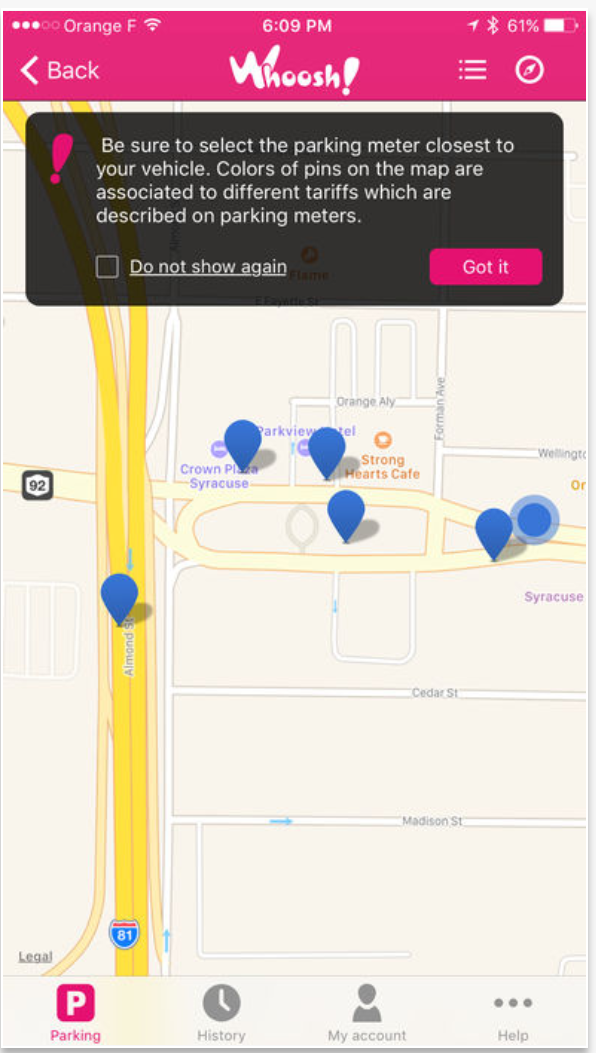
\includegraphics[scale=0.5]{img/whoosh}
				\caption{Whoosh!}
				\label{img:whoosh}
			\end{figure}
		\end{samepage}
	\newpage
	\item 
		\begin{samepage}
			PathToPark mobilioji programėlė specializuojasi navigacija iki stovėjimo aikštelių, taip pat parodo stovėjimo aikštelių laisvas vietas. Taip pat programėlė turi daug mokėjimo pasirinkimų. (2 paveikslėlis)
			\begin{figure}[H]
				\centering
				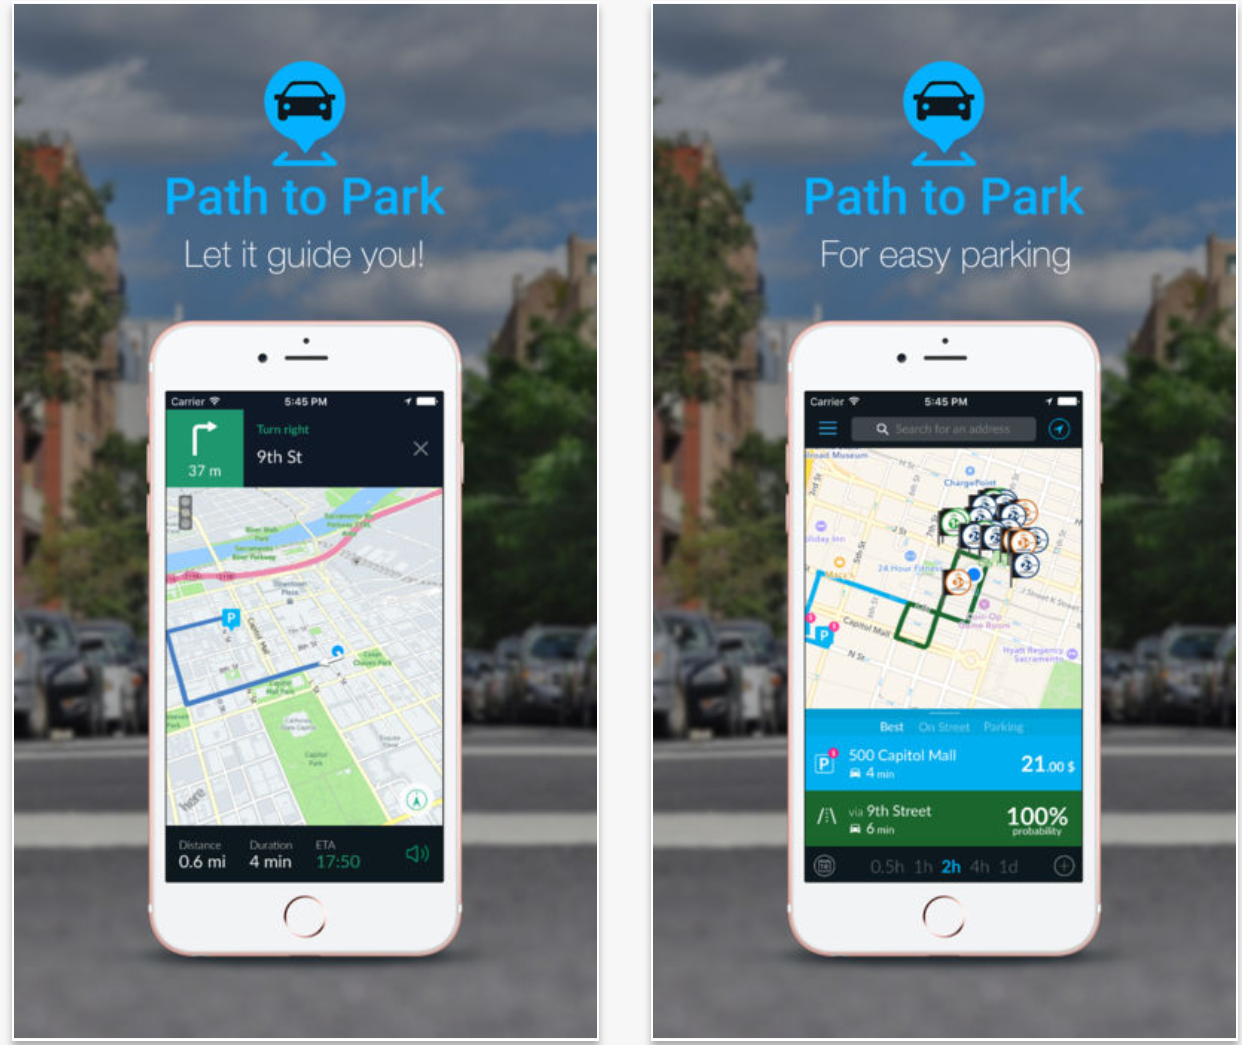
\includegraphics[scale=0.4]{img/pathtopark}
				\caption{PathToPark}
				\label{img:pathtopark}
			\end{figure}
		\end{samepage}
	\newpage
	\item
		\begin{samepage}		
			Konkurentų m.Parking mobilioji programėlė apima viso Vilniaus viešųjų stovėjimo aikštelių apmokestinimą. Jų interfeisas yra paprastas, greitas, lengvai suprantamas tiek naujam vartotojui, tiek patyrusiam. Pasirinkus automobilį, aikštelę ir stovėjimo laiką, vartotojas palenkia svirtį į priekį ir apmoka už paslaugą. (3 paveikslėlis)
			\begin{figure}[H]
				\centering
				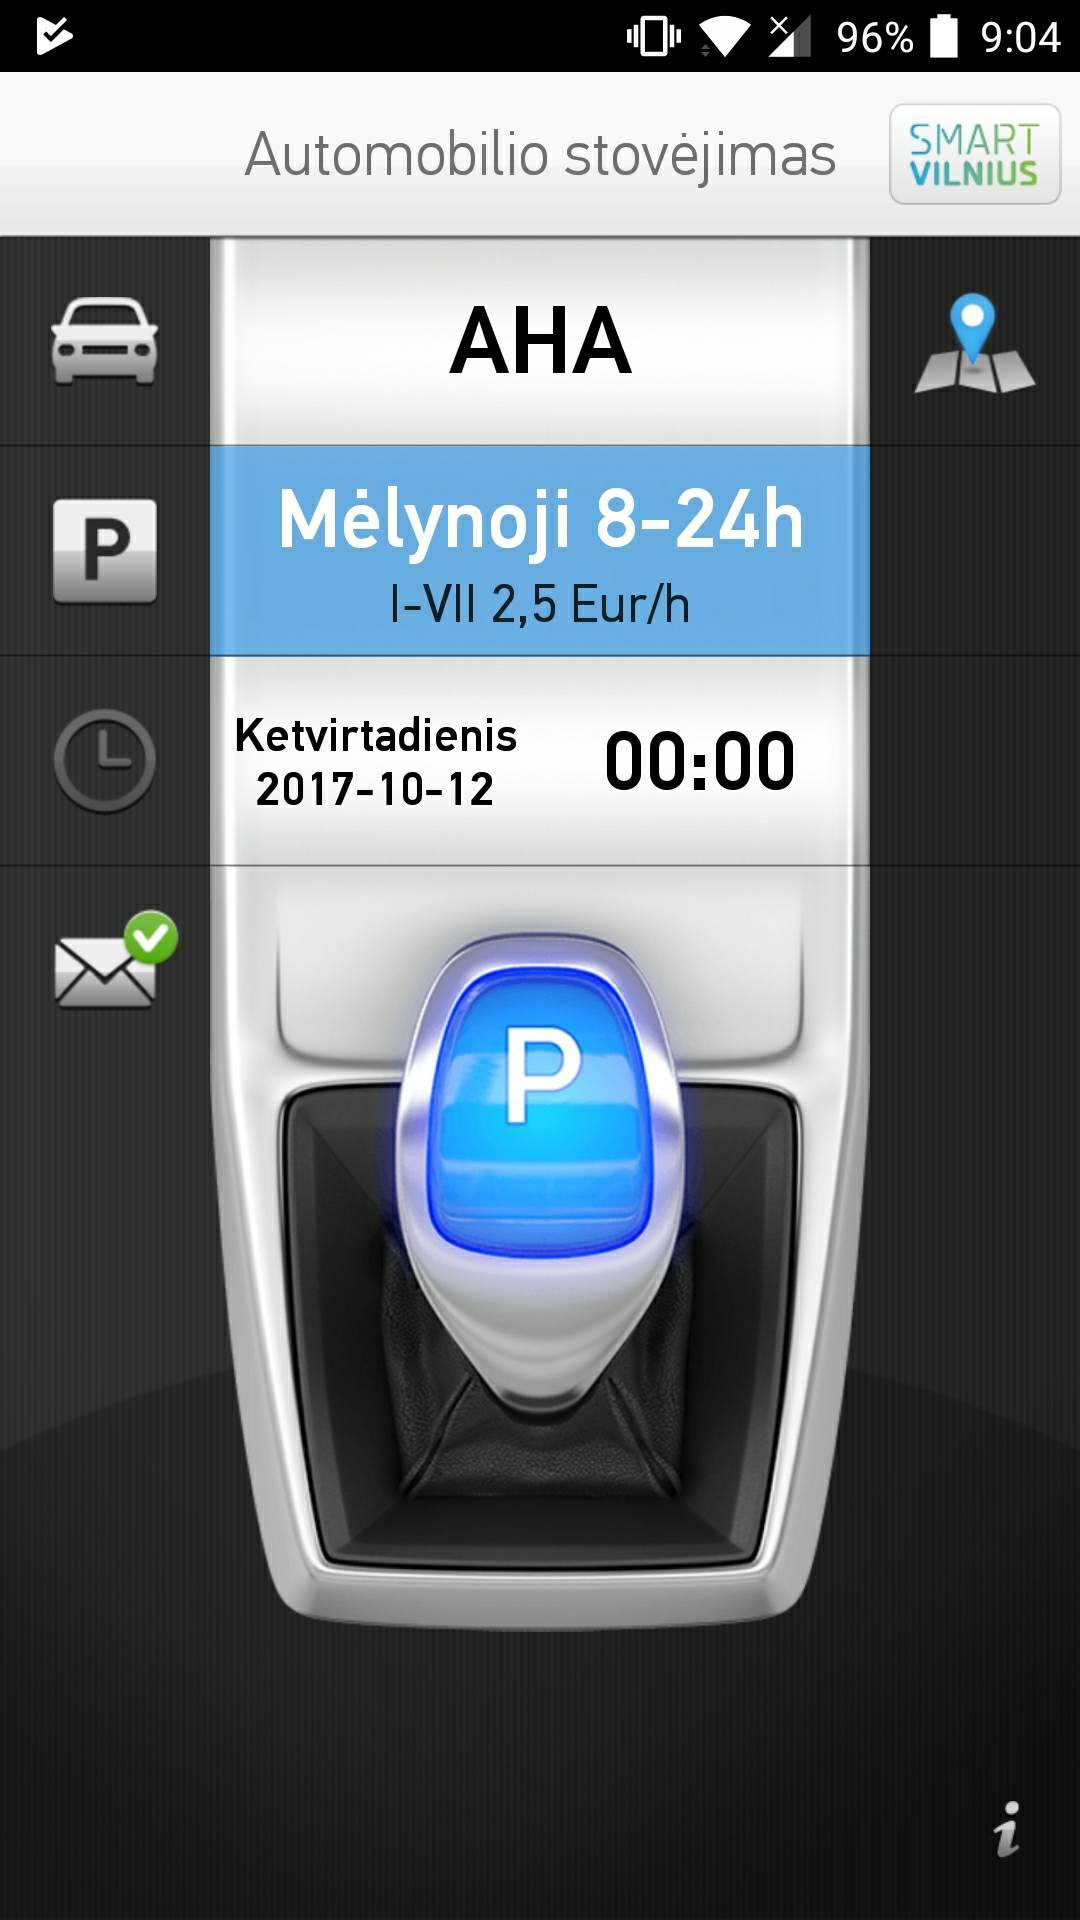
\includegraphics[scale=0.3]{img/mparking}
				\caption{m.Parking}
				\label{img:mparking}
			\end{figure}
		\end{samepage}
	\newpage
	\item
		\begin{samepage}		
			Taip pat konkurentų uniPark mobilioji programėlė, kuri naudojama apmokėti paslaugas už automobilio stovėjimą, tam tikroje uniPark aikštelėje. Jų programėlė turi galimybę parodyti žemėlapyje visas aikšteles, esančias mieste. (4 paveikslėlis)
			\begin{figure}[H]
				\centering
				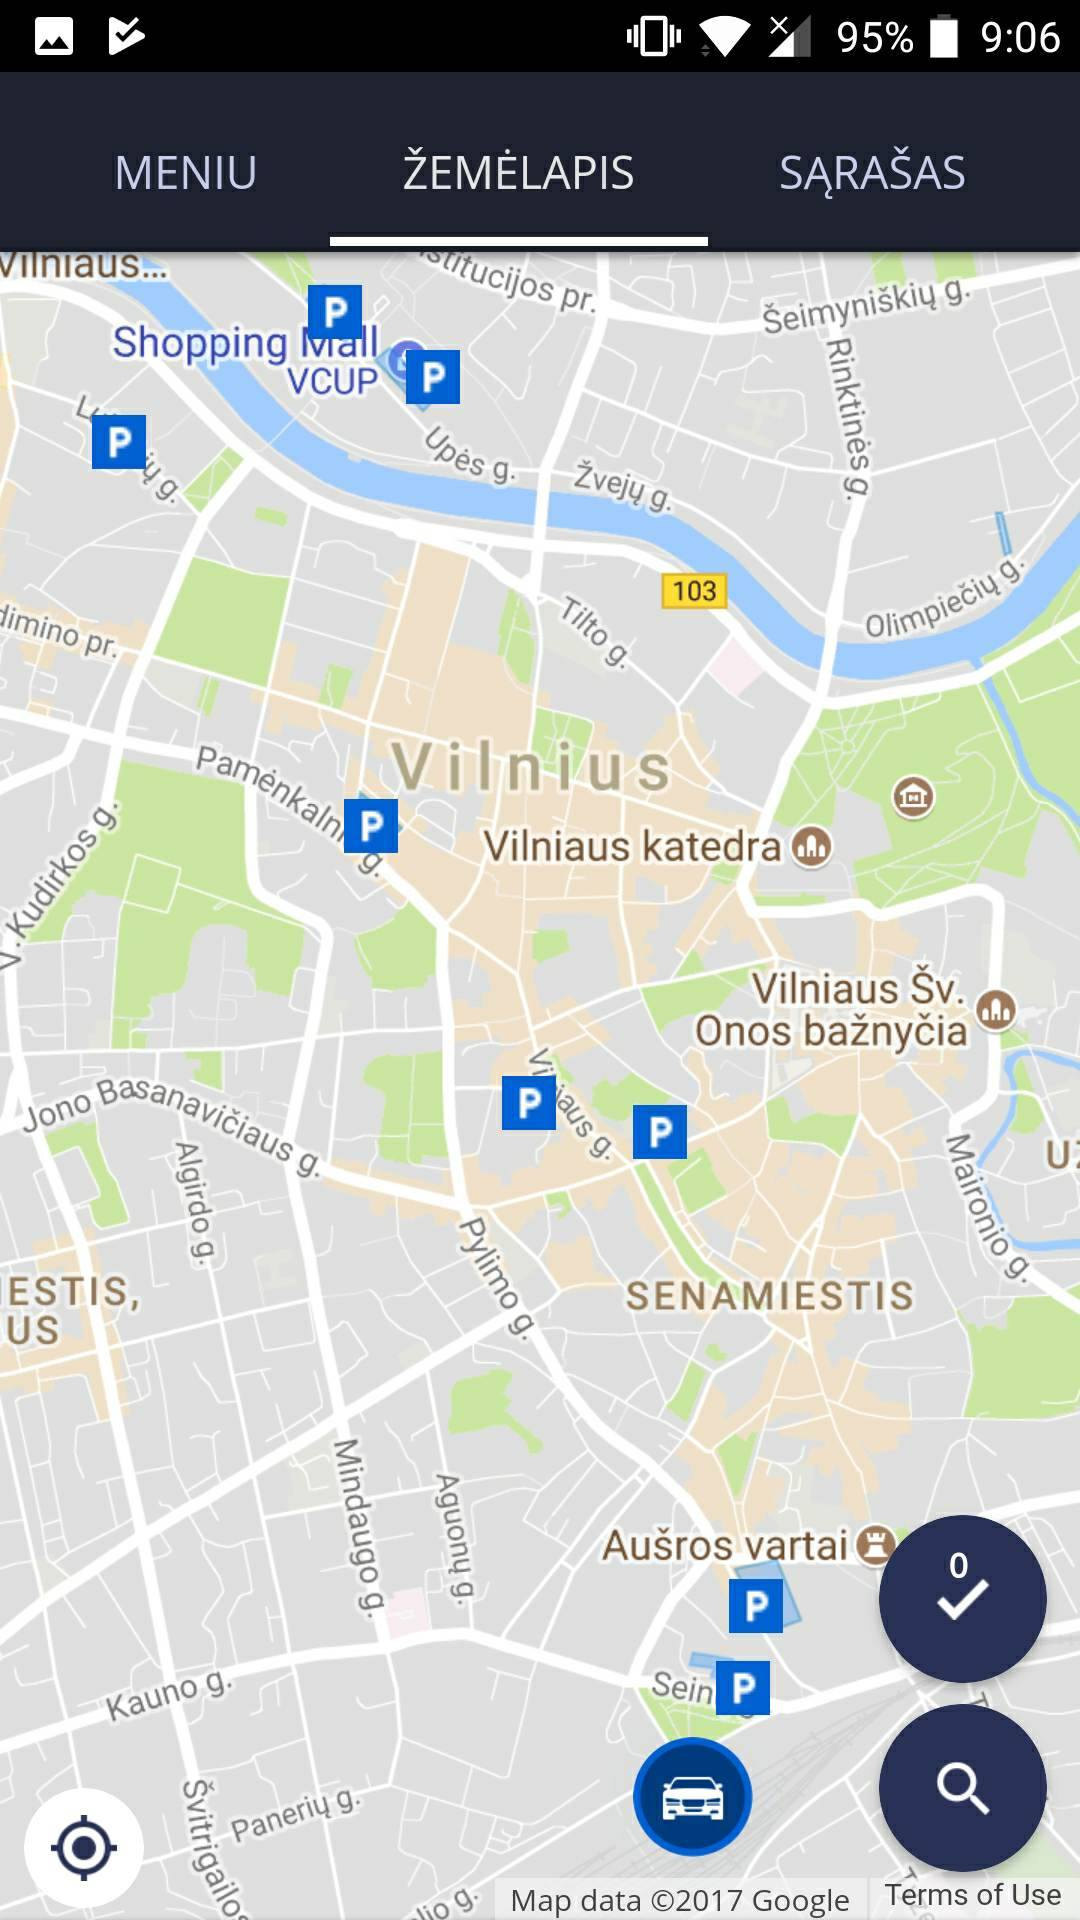
\includegraphics[scale=0.3]{img/unipark}
				\caption{uniPark}
				\label{img:unipark}
			\end{figure}
		\end{samepage}
	\item
		\begin{samepage}		
			PARK SMARTER™ mobilioji aplikacija geba greitai parodyti artimiausias laisvas parkavimo aikšteles, siunčia vartotojui realaus laiko pranešimus apie aikštelės ir rezervacjos būsenas, suteikia galimybę užregistruoti daug automobilių naudojant vieną saskaitą bei geba prisijungti naudojant integraciją su socialiniais tinklais. (5 paveikslėlis)
			\begin{figure}[H]
				\centering
				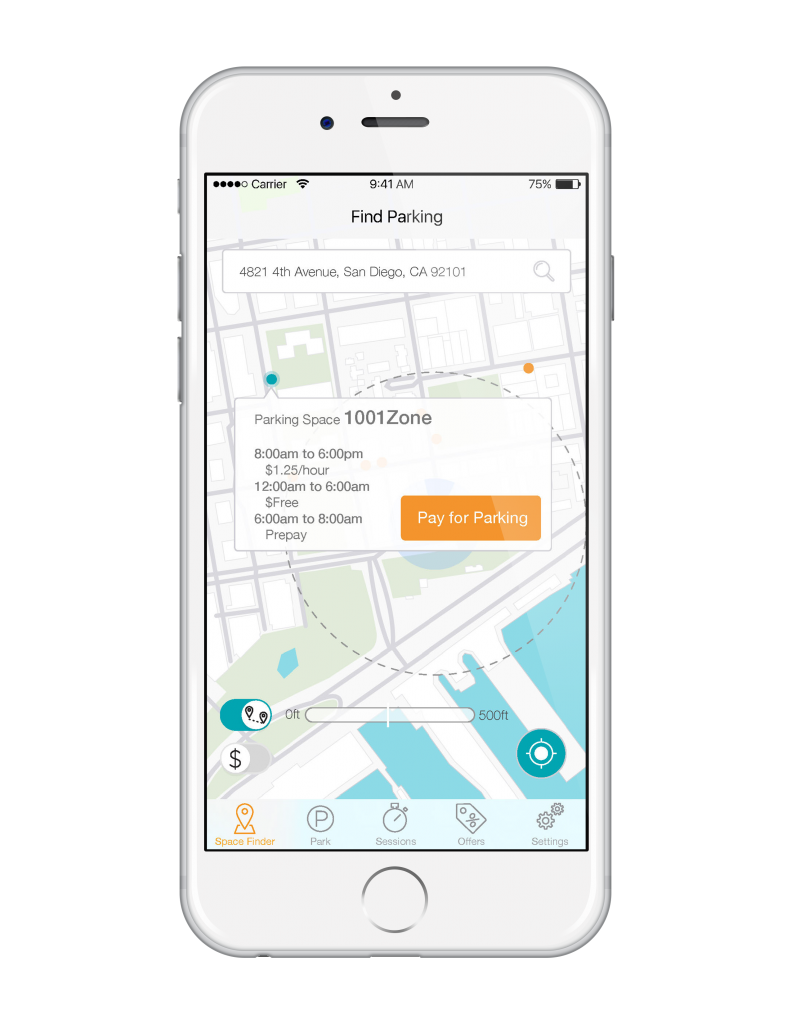
\includegraphics[scale=0.3]{img/smartpark}
				\caption{PARK SMARTER™}
				\label{img:smartpark}
			\end{figure}
		\end{samepage}
\end{enumerate}

\sectionnonum{Terminų žodynėlis}
\begin{itemize}
	\item QR kodas - optinė etiketė, sukurta iššifravimui dideliu greičiu.
	\item Vairuotojas - asmuo, kuris gali vairuoti automobilį ir naudojasi mobiliosiomis aplikacijomis.
	\item Wi-Fi internetas - belaidžio ryšio technologija leidžia realizuoti duomenų perdavimo tinklus.
	\item Išmanusis telefonas - mobilusis telefonas su operacine sistema, turintis pažangių kompiuterinių gebėjimų apdoroti duomenis ir prisijungti prie įvairių ryšių tinklų.
	\item Planšetinis kompiuteris - nešiojamas mobilusis kompiuteris su lietimui jautriu ekranu, didesnis už mobilųjį telefoną ar delninį kompiuterį.
	\item GPS - globali padėties nustatymo sistema.
	\item Parkuotis - laikyti mechanines transporto priemones tam skirtoje vietoje (stovėjimo aikštelėje).
	\item Programėlė (mobilioji programėlė, mobilioji aplikacija) - taikomoji programinė įranga, skirta išmaniesiems telefonams ir plašetiniams kompiuteriams.
	\item Mood detector - angliškas išsireiškimas, norint greitai įvertinti paslaugos veikimą pateikiant vartotojui pasirinkimą iš kelių nuotaikos būsenų.
\end{itemize}


\sectionnonum {Priedai}
	Šios analizės kūrėjai - keturi studentai, norintys pagerinti dabartinę parkavimo sistemą ne tik dėl pinigų, bet ir dėl bendro pasaulio gėrio ir Lietuvos technologinių sugebėjimų kėlimo. Visi studentai turi vairavimo teises ir pusė iš jų vairuoja beveik kasdien. Ši komanda jau 2 kurse aprašinėjo tokias sistemas kaip: ,,Festofilas'' - Festivalių megėjų puslapis, ,,LtNSO'' - Lietuvos nacionalinės sporto organizacijos sistema, ,,GSSP'' - Grupinių sporto susitikimų platforma. Todėl ši komanda tikrai pasiruošusi susidoroti su ateityje atsirandančiais iššūkiais. Šiuo metu komandai padeda dr. Kristina Lapin.
\end{document}
